\documentclass[11pt,letterpaper]{article}
\usepackage[utf8]{inputenc}
\usepackage[english]{babel}
\usepackage{titlesec}
%%%%%%%%%%%%%%%%%%%%%%%%%%%%%%%%%%%%%%%%%%%%%%%%%%%%%
\usepackage{amsmath}
\usepackage{amsfonts}
\usepackage{amssymb}
\usepackage{mathtools}
\usepackage[margin=1in]{geometry}
%%%%%%%%%%%%%%%%%%%%%%%%%%%%%%%%%%%%%%%%%%%%%%%%%%%%%
\usepackage{graphicx}
\usepackage{tikz}
\graphicspath{{./Assignment7Graphs/}}
\usetikzlibrary{calc}
\usepackage{tikz-3dplot}
%%%%%%%%%%%%%%%%%%%%%%%%%%%%%%%%%%%%%%%%%%%%%%%%%%%%%
\usepackage{varioref}
\usepackage{fancyref}
\usepackage{float}
\floatstyle{boxed}
\restylefloat{figure}
\usepackage{framed}
\usepackage{subfig}
%%%%%%%%%%%%%%%%%%%%%%%%%%%%%%%%%%%%%%%%%%%%%%%%%%%%%
\usepackage[]{algorithm2e}

\usepackage{listings}
\usepackage{color}

\titleformat{\subsection}[runin]
  {\normalfont\large\bfseries}{\thesubsection}{1em}{}
\titleformat{\subsubsection}[runin]
  {\normalfont\normalsize\bfseries}{\thesubsubsection}{1em}{}

\definecolor{dkgreen}{rgb}{0,0.6,0}
\definecolor{gray}{rgb}{0.5,0.5,0.5}
\definecolor{mauve}{rgb}{0.58,0,0.82}

\lstset{language=Java,
  aboveskip=3mm,
  belowskip=3mm,
  showstringspaces=false,
  columns=flexible,
  basicstyle={\small\ttfamily},
  numbers=none,
  numberstyle=\tiny\color{gray},
  keywordstyle=\color{blue},
  commentstyle=\color{dkgreen},
  stringstyle=\color{mauve},
  breaklines=true,
  breakatwhitespace=true,
  tabsize=3
}
%%%%%%%%%%%%%%%%%%%%%%%%%%%%%%%%%%%%%%%%%%%%%%%%%%%%%
%Script R%
\usepackage{calligra}
\usepackage{qtree}
\DeclareMathAlphabet{\mathcalligra}{T1}{calligra}{m}{n}
\DeclareFontShape{T1}{calligra}{m}{n}{<->s*[2.2]callig15}{}
\newcommand{\scripty}[1]{\ensuremath{\mathcalligra{#1}}}
\newcommand{\sr}{\scripty{r}}
\newcommand{\vsr}{\vec{\sr\,}}
%%%%%%%%%%%%%%%%%%%%%%%%%%%%%%%%%%%%%%%%%%%%%%%%%%%%%
%Macros%
\newcommand{\dint}[2]{\int\limits_{#1}^{#2}}

%%%%%%%%%%%%%%%%%%%%%%%%%%%%%%%%%%%%%%%%%%%%%%%%%%%%%
\author{Alex Pizzuto}
\title{CS 577 Homework 7}
\begin{document}
\date{}
\maketitle
\hrule

\section*{Question One: Maximum flow minimum cut problem}
We are given the following graph, and asked to find the maximum flow: 

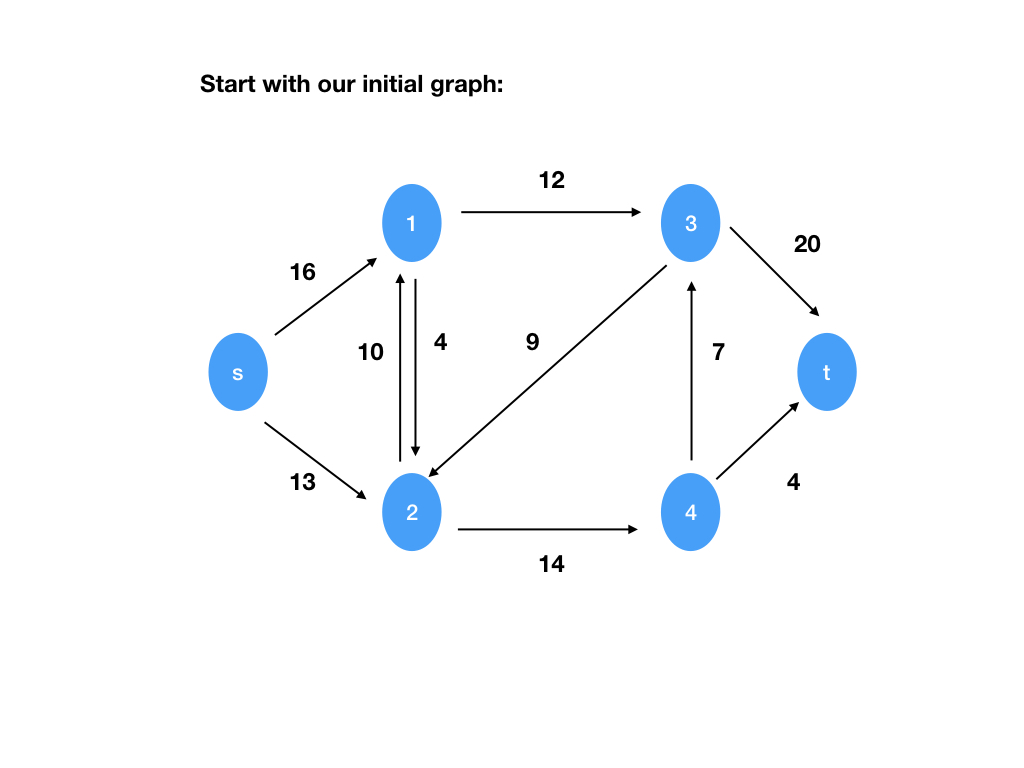
\includegraphics[width=10cm]{Graph1.jpeg}

We include all major subsequent steps with labels. We will use red to label backwards edges and black to denote forwards edges. The different colors used are to highlight specific nodes being considered for a given augmented path. The final max flow diagram is just the final residual graph where all backwards edges represent the forward flow through them. 

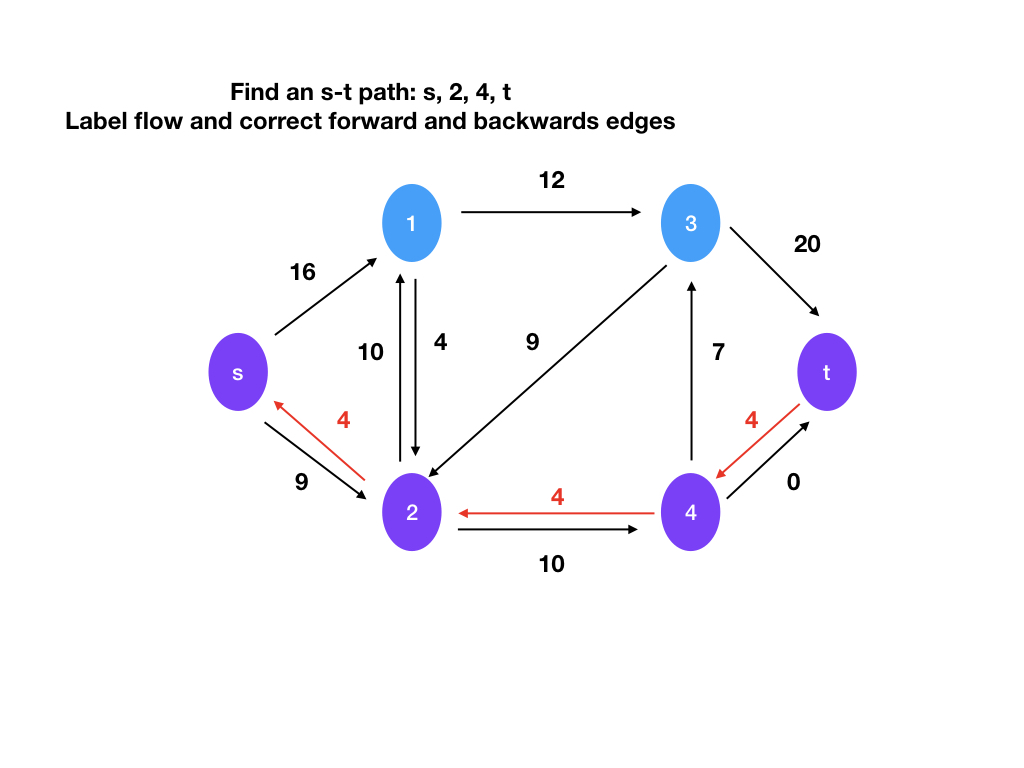
\includegraphics[width=10cm]{Graph2.jpeg}

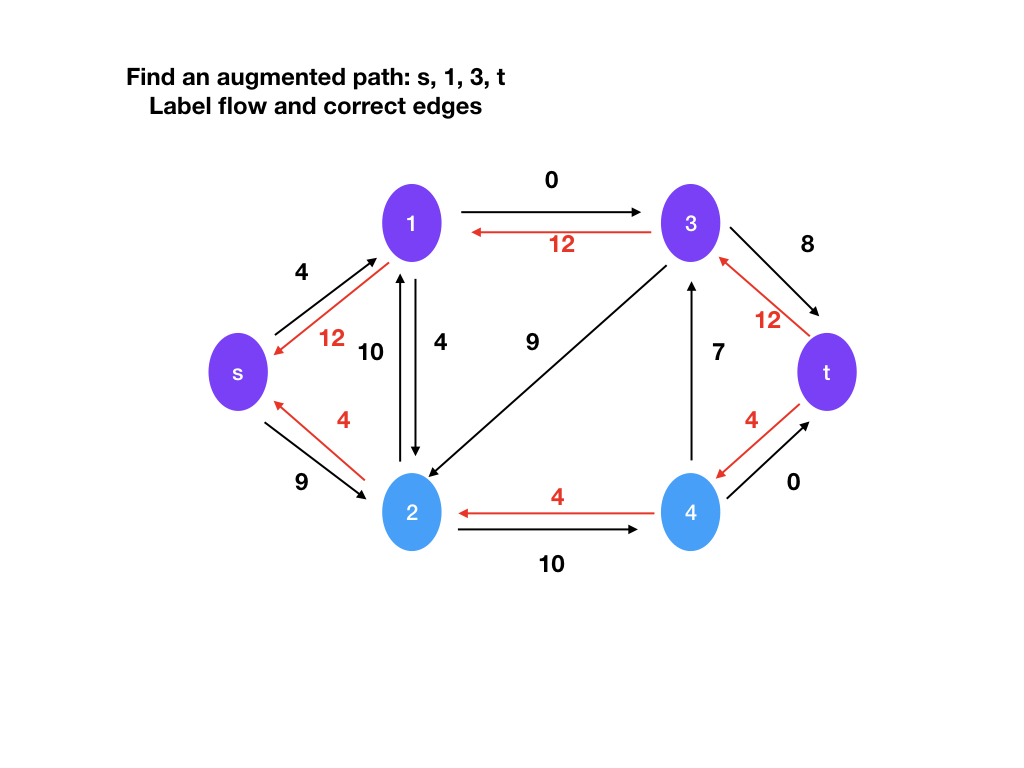
\includegraphics[width=10cm]{Graph3.jpeg}

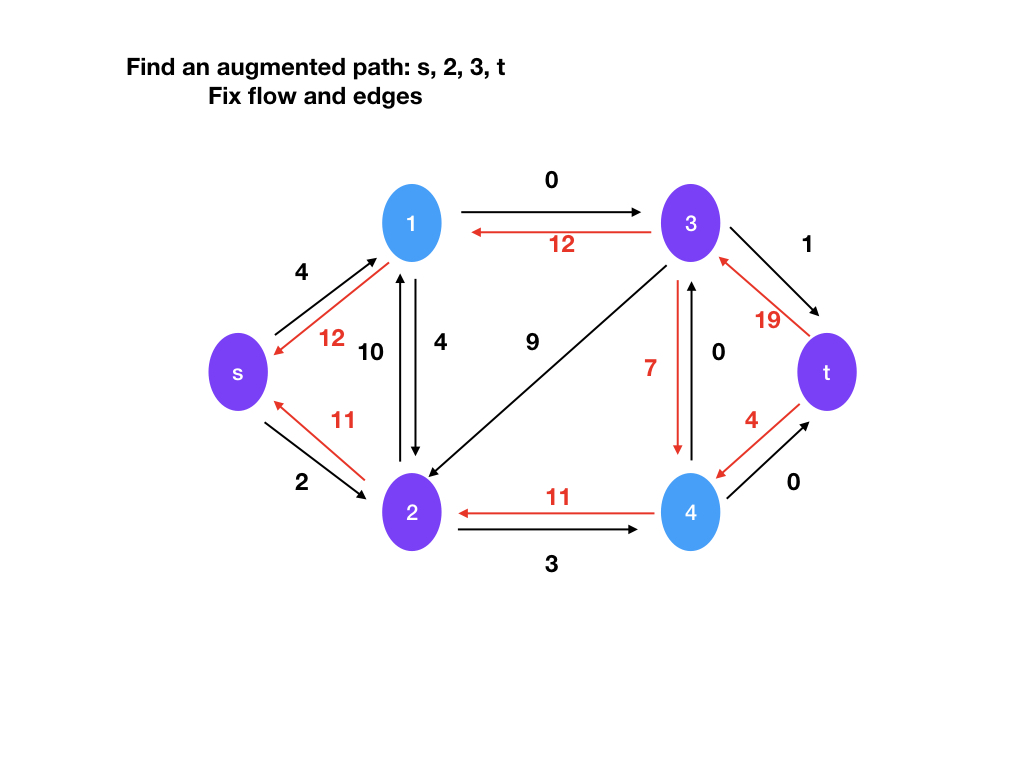
\includegraphics[width=10cm]{Graph4.jpeg}

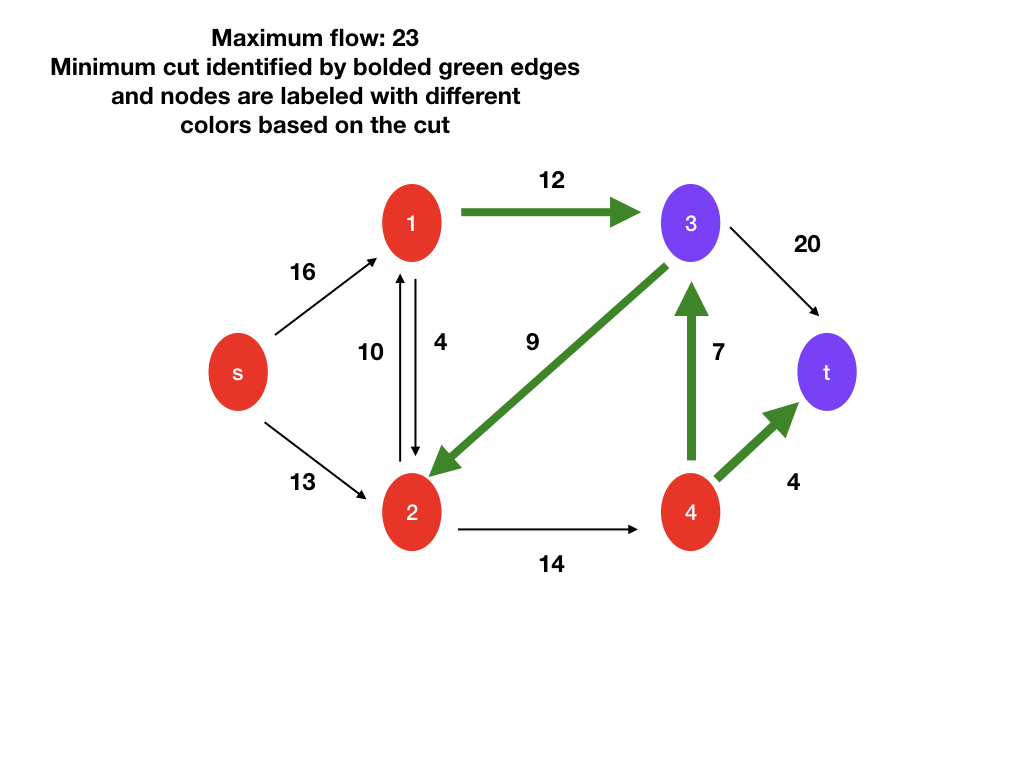
\includegraphics[width=10cm]{Graph5.jpeg}

\section*{Question Two: 7.9}
In order to determine whether or not we can distribute all of the patients to all of the hospitals such that each hospital has at most $\lceil n/k \rceil$ people, consider the following flow network. First, we create a node for every patient, $i$ and one for every hospital, $j$. Then, if patient $i$ is within a half-hour's drive from hospital $j$, we connect these two nodes with an edge of capacity 1. Then, we create one parent source node, $s$, and one final sink node, $t$. We connect all patient nodes, $i$, to $s$ with an edge of capacity 1, and connect all hospital nodes, $j$, to $t$ with an edge of capacity $\lceil n/k \rceil$:

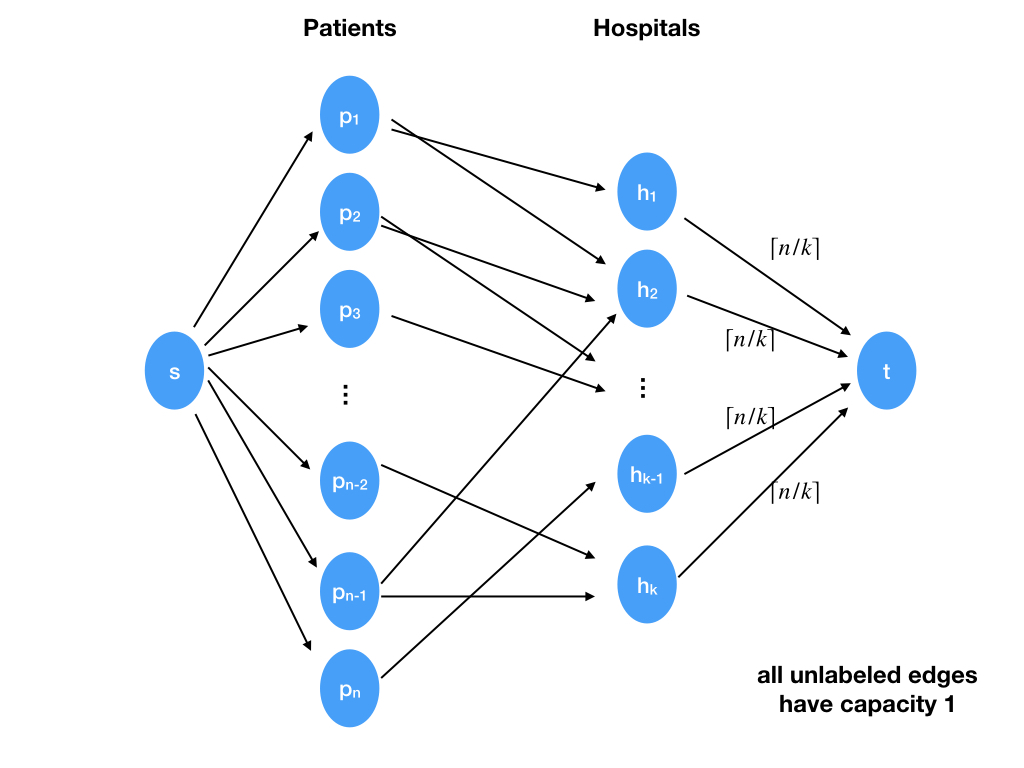
\includegraphics[width=10cm]{question79.jpeg}

Then we claim that there is a way to distribute the patients if and only if we can find an $s-t$ flow of value $n$. We would find such a path, if it exists, using the Ford-Fulkerson algorithm. We would send each patient to whichever hospital there is an edge between after the minimum cut has been determined, and we know that no hospital will be overloaded because the hospital nodes are divergenceless and the capacity to $t$ ensures that we will not send too many patients to one hospital. We know that in general, the Ford-Fulkerson algorithm runs in time $\mathcal{O}(mC)$, where $C$ is the sum of all edge costs coming out of $s$, which in this problem is $n$. Here, we have $n+k$ nodes and up to order $nk$ edges. Thus, our algorithm is polynomial as it will run in $\mathcal{O}(n^2k)$.


\section*{Question Three: 7.26}

Our algorithm will work as follows. First we construct a graph consisting of a source node, $s$, $n$ phone nodes, $p_i$,  $n$ base nodes, $b_i$, and one sink node, $t$. Then, we connect all phone nodes to the source, all base nodes to the sink, and for a given moment of time, there exists an edge $e = (p_i, b_j)$ if and only if the distance between $p_i$ and $b_j$ is less than $\Delta$. All edges have capacity 1. 

\begin{figure}[h]
  \centering
  {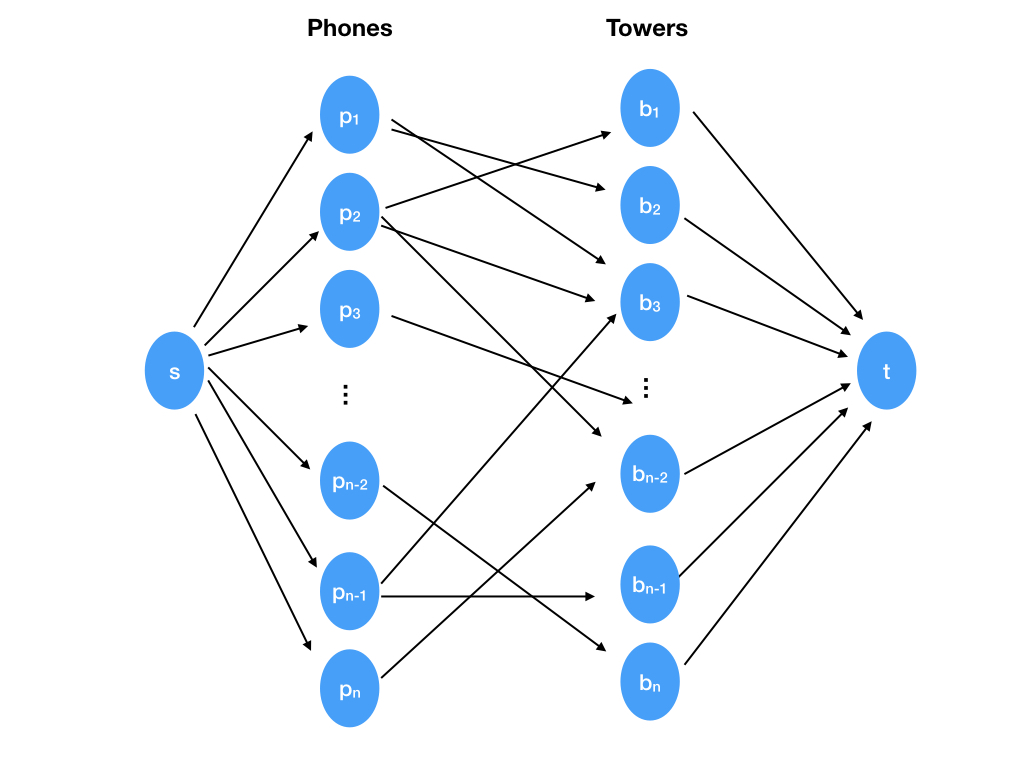
\includegraphics[width=0.4\textwidth]{726_1.jpeg}
  \hfill
  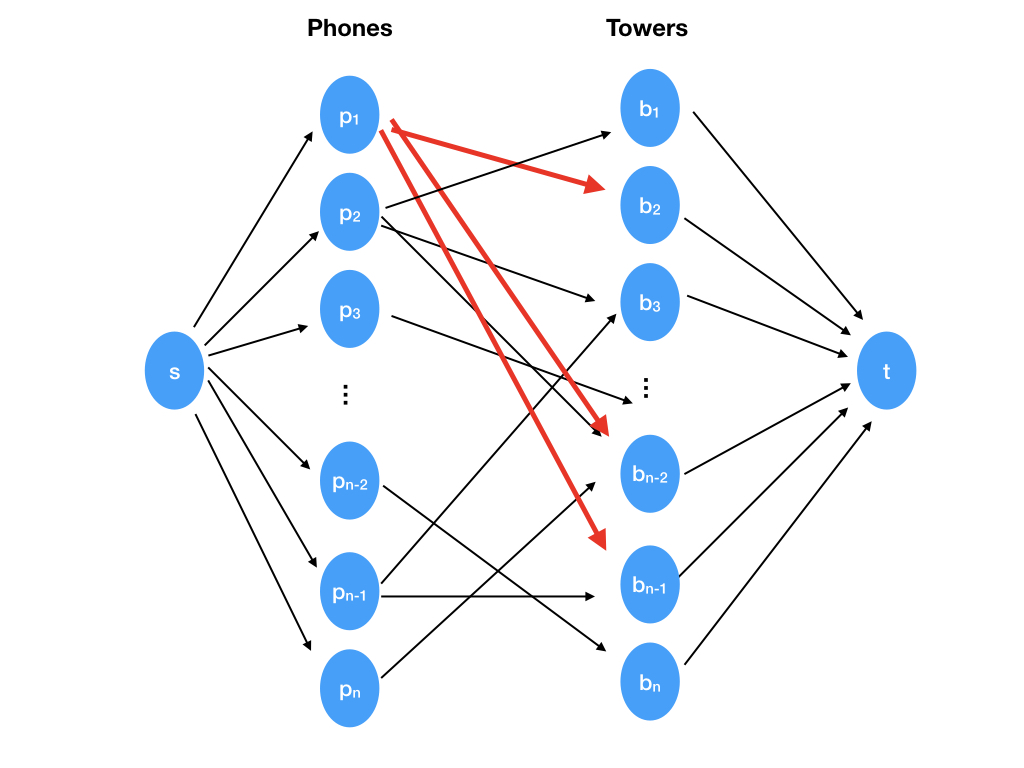
\includegraphics[width=0.4\textwidth]{726_2.jpeg}\label{fig:f2}}
  \caption{Possible evolution of graphs from one moment in time to another}
\end{figure}

Then our algorithm will run by first creating this graph for the initial time. Then, by use of the Ford-Fulkerson Algorithm, we will see if we can find a maximum flow of this graph that is equal to $n$. If this is the case, then we have flow through all of the phone and base nodes, and our conditions are met. In this case, we find the edge connecting the phone that is traveling and the base that it is using by finding our minimum cut. We continue in time until the phone that is moving loses the edge that it is currently utilizing. Then, with our new graph, we instead of rerunning the entire Ford-Fulkerson algorithm, we keep all flows as they were except for the one that was going through the phone that was moving and has been eliminated. We then take the graph that we have as our basis residual graph, and look for an augmenting path that will go through the node the lost the connection. If such an augmenting path exists and we will resume the Ford-Fulkerson algorithm from this step to see if we can find a max flow of $n$ as before. We continue doing this until either we have reached our destination, or until there is a moment when we cannot find a max flow of $n$, in which case there is no possible arrangement with full connectivity the entire time. This algorithm is bounded by the number times we must recalculate our graphs (the number of times the moving phone loses connection with its current base), which we can treat as a constant. In that case, our algorithm is bounded by the running time of the Ford-Fulkerson Algorithm combined with the running time of finding a minimum cut after this algorithm completes, with order $n$ edges. Thus, our algorithm will run in $\mathcal{O}(n^3)$ time. 


\end{document}